\documentclass[11pt]{beamer}

% Specify theme
\usetheme{PomonaMath}

\usepackage{amsmath}
\usepackage{graphicx}
\usepackage{color}
\usepackage{bbm}


\newcommand{\Rr}{\mathbb{R}}
\newcommand{\Cc}{\mathbb{C}}
\newcommand{\Nnn}{{\bf N}}
\newenvironment{greytext}{\color{gray}}{\ignorespacesafterend}
\newcommand{\indic}{\mathbbm{1}_M}
\newcommand{\SMR}{\mathrm{SMR}}
\newcommand{\race}{\texttt{race}}
\newcommand{\rrr}{\texttt{r}}
\newcommand{\varr}{\texttt{var}}


 %\setbeamertemplate{footline}[frame number]{} % Uncomment this line if you want to remove the footer from each slide (and replace it with just the slide number (X/Y) in the bottom right of each slide).

\title[Implications of Missing Traffic Stop Data]{Implications of Missing Traffic Stop Data}
% Remember to include both a short and a full title!
% The short title appears at the bottom of each slide.
\author{Amber Lee advised by Jo Hardin}
\institute[]{Pomona College}
\date{November 5, 2021}



%  \usepackage[sfmath]{kpfonts}
%  \renewcommand*\familydefault{\sfdefault}

%\setbeamerfont{frametitle}{shape=\scshape}

%%% finish
% Example -- all. bc the alignment is kind of trash
% Conclusion

%===============================================================%
\begin{document}
%===============================================================%

\maketitle


\begin{frame}{Motivation}
    Concern over racial profiling has led to mass collection of traffic stop data. As the data has been made available to the public, researchers have modeled the data to look for evidence of discrimination. \pause
    \begin{itemize}
    \item Most statistical models do not handle missing values, so most studies simply use complete-case analysis (\texttt{na.rm = True}).
    \item Chanin and Welsh (2020) draw attention to the issue of (non-random) missing values.
    % and hypothesize that officers are not incentivized to accurately and comprehensively collect data.
    \end{itemize} \pause
    $\Rightarrow$ {\bf{What are the trends of missing values in traffic stop data?}}
\end{frame}

\section{Definitions}

\begin{frame}{Row-wise missingness} %
    Let $X = (x_{ij})$ be a {\bf{dataset}} with $n$ observations and $k$ variables. 
    \begin{itemize}
    \item Each observation $i = 1, 2, \ldots, n$ represents a single traffic stop. 
    \item We denote a {\bf{missingness indicator function}} as
    % describe what a dataset is?
    \begin{equation*}
    \indic(x_{ij}) =
    \begin{cases}
    1 & \text{if $x_{ij}$ is missing} \\
    0 & \text{if $x_{ij}$ is observed}
    \end{cases}
    \end{equation*}
    \end{itemize} \pause
    \begin{definition}
    The {\bf{stop missingness rate for observation $i$}} (or row-wise $\SMR$) is the percentage of missing values for a single traffic stop $i$. 
    \begin{equation*}
    \SMR_i = \dfrac{1}{k} \sum_{j = 1}^{k} \indic(x_{ij})
    \end{equation*}
    \end{definition}
\end{frame}

%\begin{frame}{Row-wise missingness} %
%    \begin{definition}
%    The {\bf{stop missingness rate for observation $i$}} (or row-wise $\SMR$) is the percentage of missing values for a single traffic stop $i$. 
%    \begin{equation*}
%    \SMR_i = \dfrac{1}{k} \sum_{j = 1}^{k} \indic(x_{ij})
%    \end{equation*}
%    \end{definition}
%    Example
%    % insert graphic here
%    \begin{align*}
%    \SMR_1 &= 1/2 \\
%    \SMR_2 &= 3/4
%    \end{align*}
%\end{frame}

\begin{frame}{Dataset missingness}
    \begin{definition}
    The {\bf{stop missingness rate for dataset $X$}} (or dataset $\SMR$) is the percentage of missing values in the entire dataset. Equivalently, it is the average row-wise missingness. 
    \begin{equation*}
    \SMR(X) = \dfrac{1}{n} \sum_{i = 1}^{n} \SMR_i
    \end{equation*}
    \end{definition} \pause
    \begin{columns}
        \column{0.3\textwidth}
        Example
            \begin{equation*}
    	    \SMR(X) = 2/16
	    \end{equation*}
    \column{0.7\textwidth}
	    \begin{center}
	    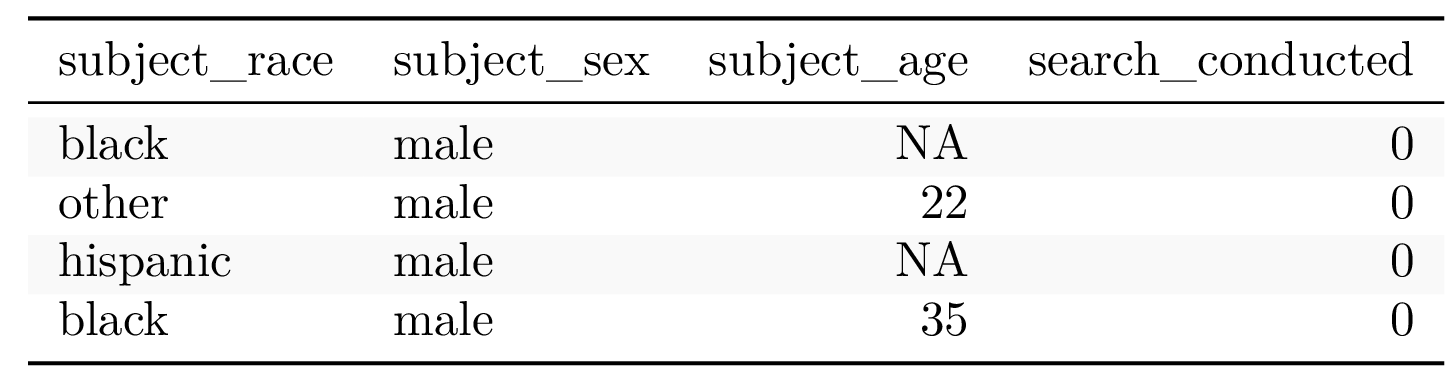
\includegraphics[scale = 0.6]{fig/toyoak.png}
	    \end{center}
    \end{columns}
\end{frame}

\begin{frame}{Missingness by a variable}
    % One limitation of $\SMR_i$ and $\SMR(X)$ is that we can't see how missingness varies \emph{by} a variable, like time of day or the \race \, of the driver. 
    \begin{definition}
    The {\bf{$\SMR$ for observation $i$ restricted by variable $j'$}} is the percentage of missing values for a traffic stop $i$, excluding variable $j'$. 
    \\~\\
    Let $j' \in \{1, 2, \ldots, k\}$ be the column index for a variable of interest. The SMR for observation $i$ restricted by $j'$ is given by
    \begin{equation*}
    \SMR_{i, j'} = \dfrac{1}{k-1} \sum_{j \neq j'} \indic(x_{ij}).
    \end{equation*}
    \end{definition} \pause
    \begin{columns}
        \column{0.3\textwidth}
        Example
            \begin{gather*}
    	    \SMR_{1, \texttt{race}} = 1/3 \\
	    \SMR_{2, \texttt{race}} = 0 \\
	    \end{gather*}
    \column{0.7\textwidth}
	    \begin{center}
	    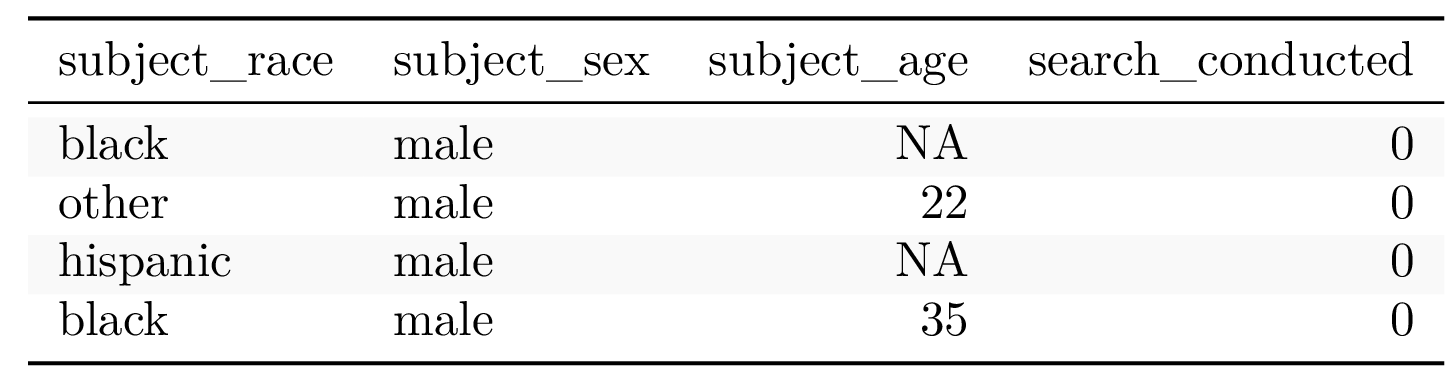
\includegraphics[scale = 0.6]{fig/toyoak.png}
	    \end{center}
    \end{columns}
\end{frame}

\begin{frame}{SMR by \race}
    Let's quantify how missingness varies by \race. 
    \\~\\
    Let $\rrr \in \{ 1, 2, \ldots, k \}$ be the column index corresponding to the \race \,  variable in $X$. 
    \\~\\
    Assume that $(x_{i, \rrr})$ has only three levels: ``White", ``Other", and \texttt{NA} (missing). We can partition the observations into index sets $(W)$, $(O)$, and $(\texttt{NA}) \subseteq \{1, 2, \ldots, n\}$ such that
    \begin{equation*}
    x_{i, \rrr} =
    \begin{cases}
    	\text{``White"} & i \in (W) \\
	\text{``Other"} & i \in (O) \\
	\, \texttt{NA} & i \in (\texttt{NA}).
    \end{cases}
    \end{equation*}
\end{frame}

\begin{frame}{SMR by \race}
    The White-$\SMR$, Other-$\SMR$, and \texttt{NA}-$\SMR$ are given by:
    \begin{align*}
    &\SMR_{(W)} = \dfrac{1}{ |(W)| } \sum_{i \in (W)} \SMR_{i, \rrr} \\
    &\SMR_{(O)} = \dfrac{1}{ |(O)| } \sum_{i \in (O)} \SMR_{i, \rrr} \\
    &\SMR_{(\texttt{NA})} = \dfrac{1}{ |(\texttt{NA})| } \sum_{i \in (\texttt{NA})} \SMR_{i, \rrr}.
    \end{align*}
    \begin{columns}
        \column{0.3\textwidth}
        Example
            \begin{gather*}
    	    \SMR_{(B)} = 1/6 \\
	    \SMR_{(H)} = 1/3 \\
	    \SMR_{(O)} = 0 \\
	    \end{gather*}
    \column{0.7\textwidth}
	    \begin{center}
	    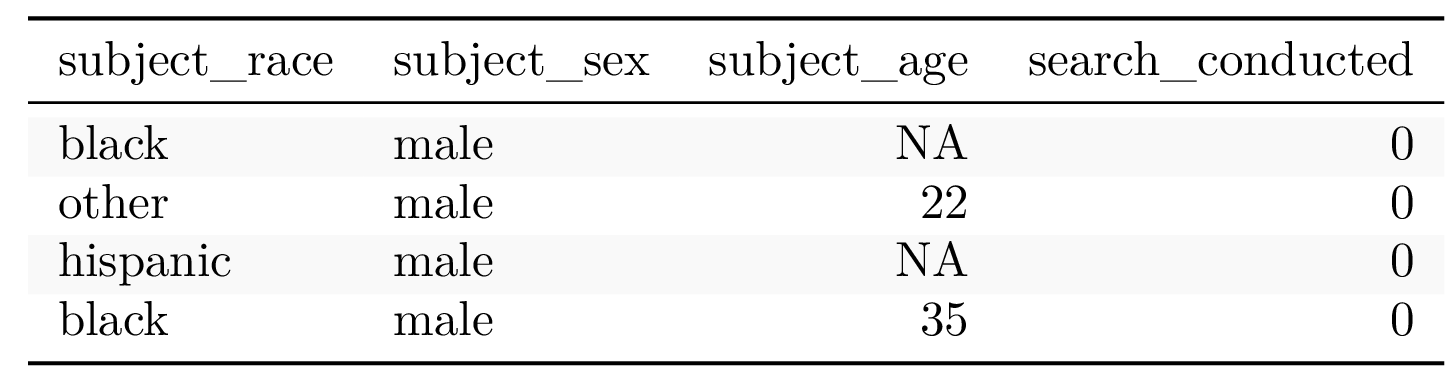
\includegraphics[scale = 0.6]{fig/toyoak.png}
	    \end{center}
    \end{columns}
\end{frame}

\begin{frame}{SMR by \texttt{date} and \texttt{time}}
	We apply a similar method to continuous variables.
	\\~\\
	We need to be careful with partitioning the indices -- the partitions need enough observations for the average restricted $\SMR$s to be meaningful.
	\\~\\ \pause
	\begin{itemize}
	\item For \texttt{date}, we partition observations by the week.
	\item For \texttt{time}, we partition observations by the month and day/night.
	\end{itemize}
	
	
	
\end{frame}

%\begin{frame}{Generalizing SMR by \race}
%    \begin{definition}
%    Let $\varr \in \{1, 2, \ldots, k \}$ be a column index for a variable $x_{i, \varr}$ that has possible values $s_1, s_2, \ldots, s_m$. We create with index sets $(S_1), (S_2), \ldots, (S_m)$ to partition $X$ satisfying
%    \begin{equation*}
%    x_{i, \varr} = s_\ell \text{ for $1 \leq \ell \leq m$ and all $i \in S_\ell$.}
%    \end{equation*} \pause
%    The {\bf{$s_\ell$-$\SMR$}} is the percentage of missing values, not including \varr, when $x_{i, \varr} = s_\ell$. Equivalently, the $s_\ell$-$\SMR$ is the average restricted SMR for \varr \, over $i \in (S_\ell)$.
%    \begin{equation*}
%    \SMR_{(S_\ell)} = \dfrac{1}{| (S_\ell) |} \sum_{i \in S_\ell} \SMR_{i, \varr}
%    \end{equation*}
%    \end{definition} \pause
%    This will be helpful for variables \race, \texttt{date}, and \texttt{time}. 
%\end{frame}

\section{About the data}

\begin{frame}{About the datasets}
    The Stanford Open Policing Project several dozen datasets from 1999 to 2020. Each dataset records a different set of variables. \pause
    	\vspace{1ex}
	\begin{center}
	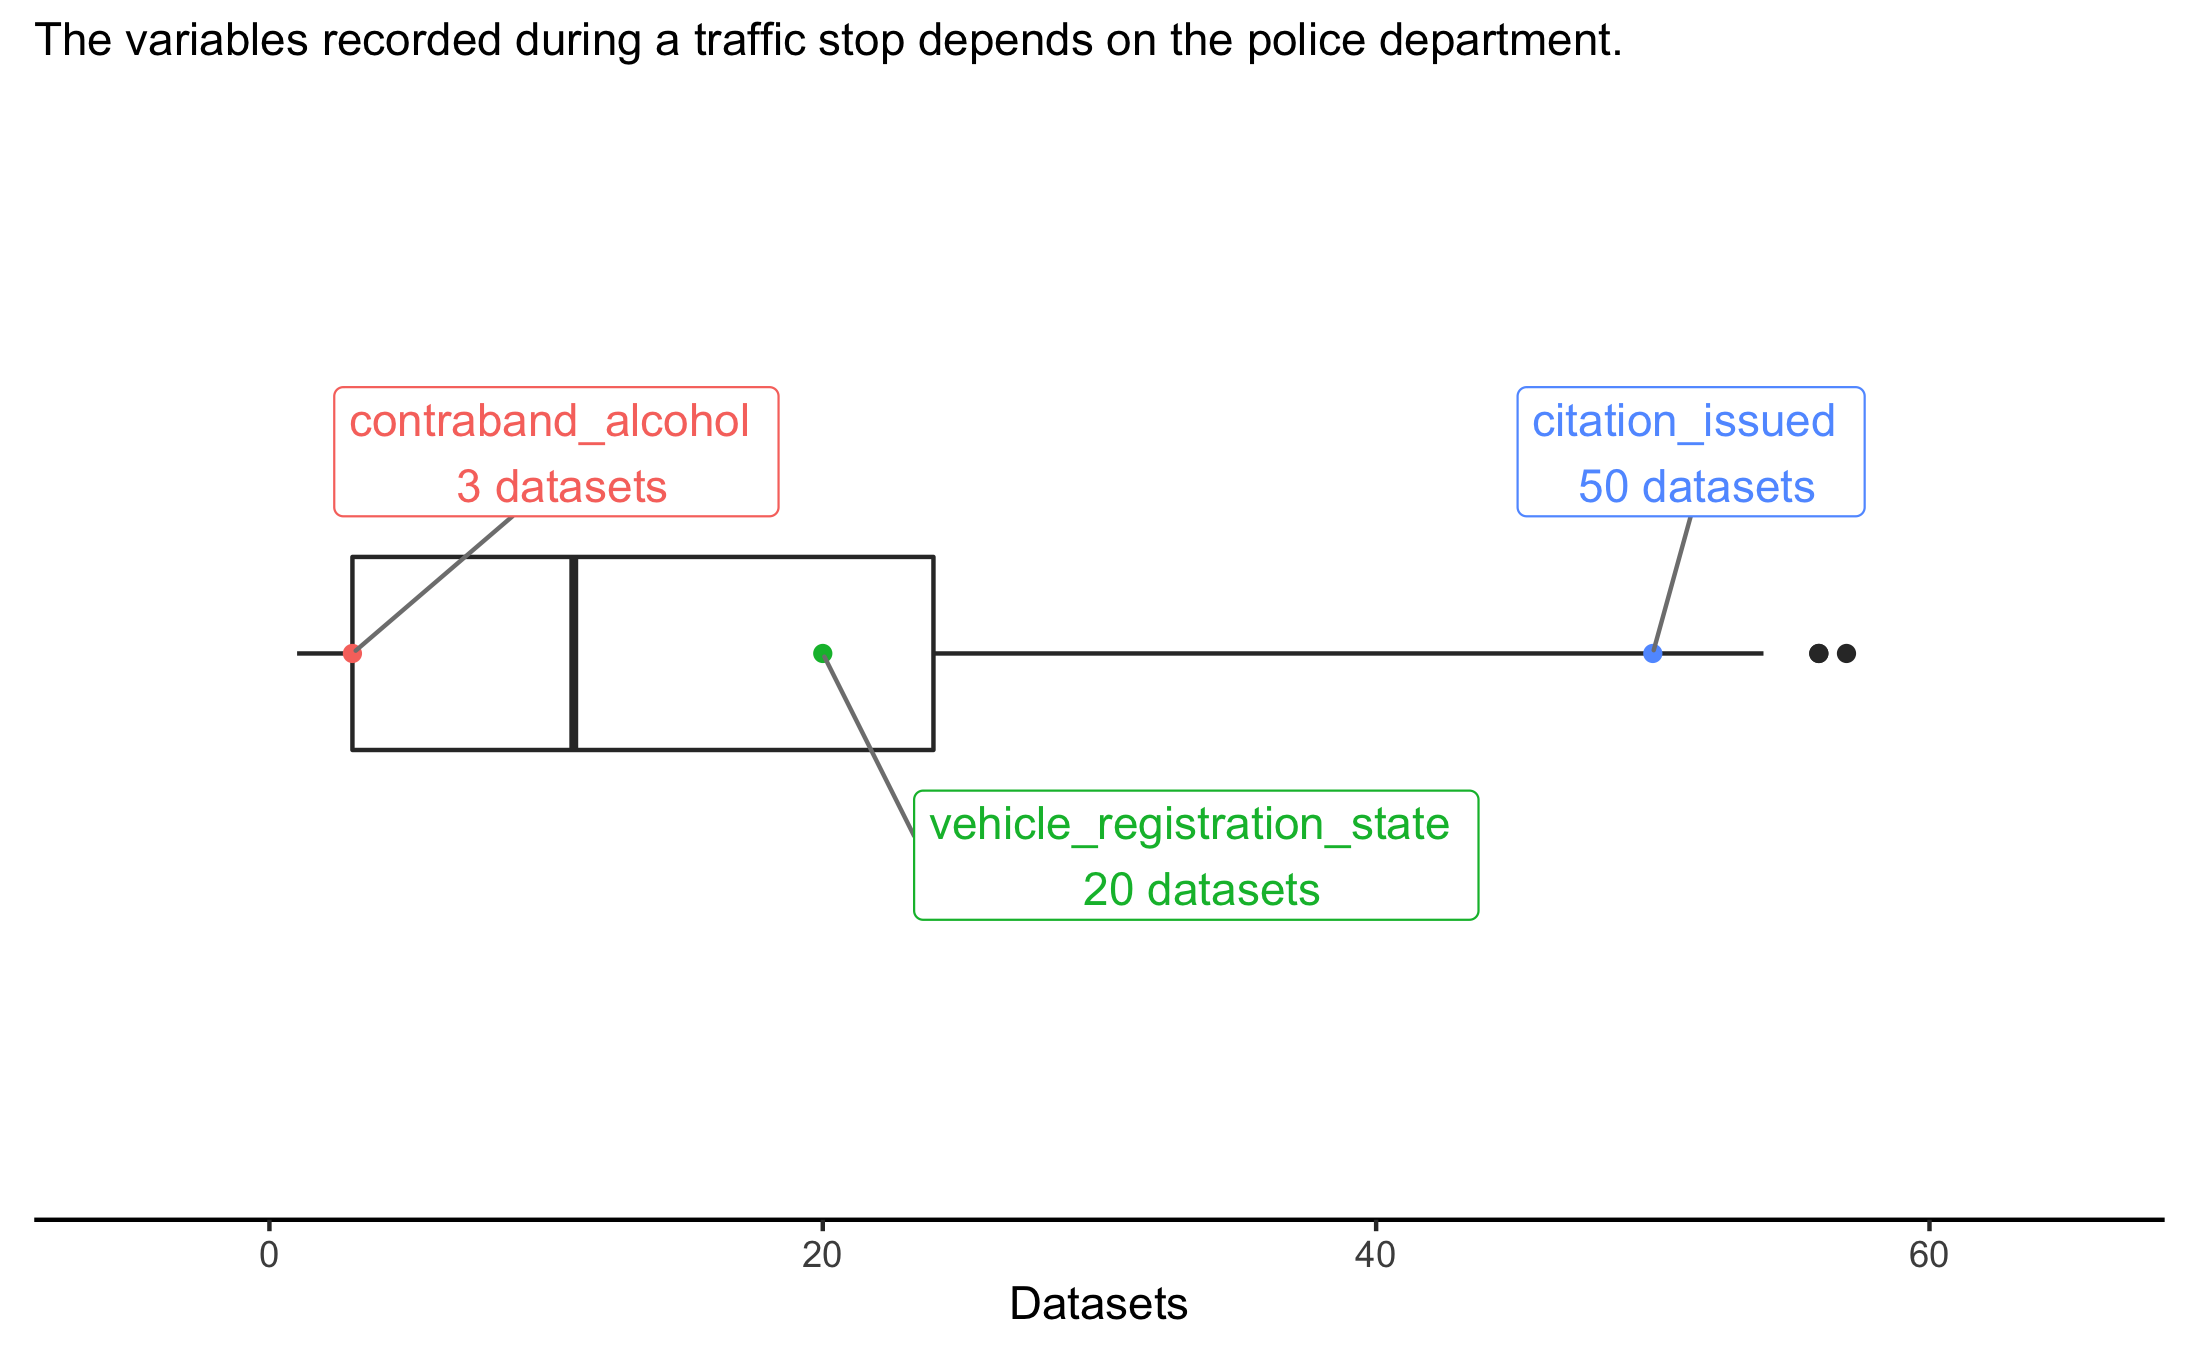
\includegraphics[scale=0.1]{fig/var_dist.png}
	\end{center} 
\end{frame}

%\begin{frame}{About the datasets}
%      \begin{center}
%      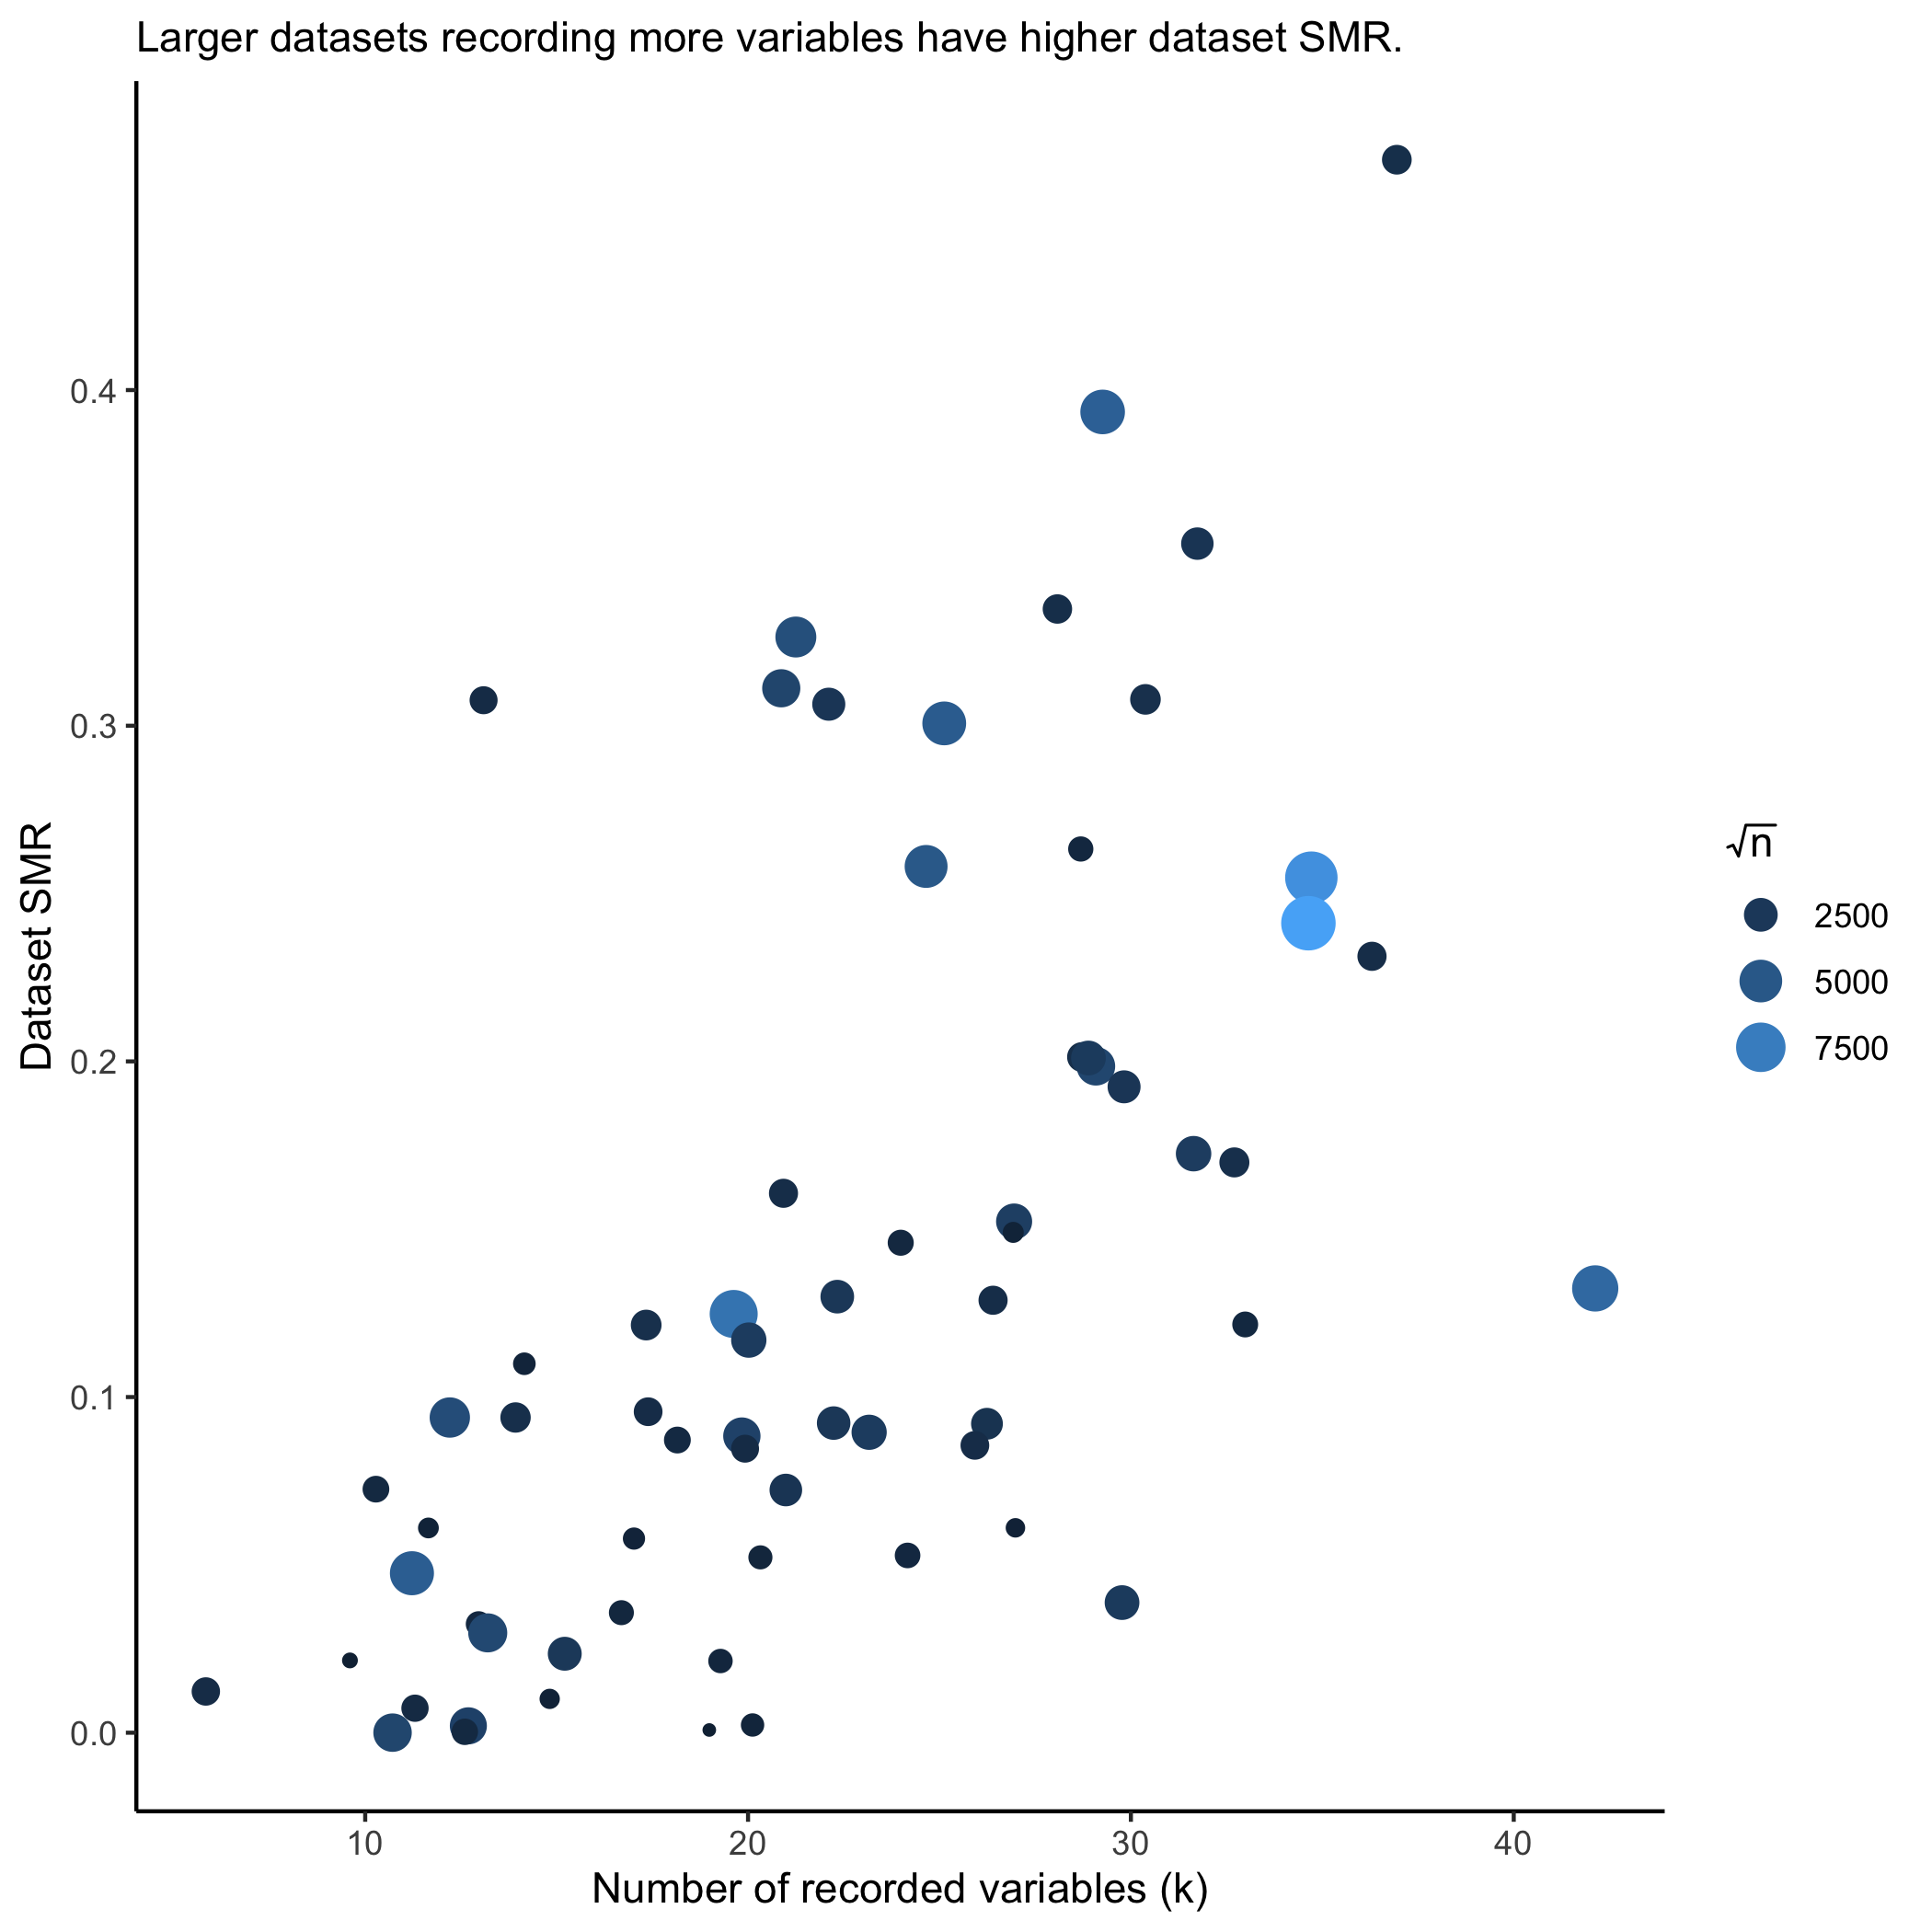
\includegraphics[scale = 0.1]{fig/SMR_n_k.png}
%      \end{center}
%\end{frame}

\begin{frame}{Data pre-processing}
	% datasets collect
	We select $k = 9$ variables about 
	\begin{itemize} 
	\item driver demographic: \texttt{race}, \texttt{sex}, \texttt{age};
	\item situational details: \texttt{time}, \texttt{date}, \texttt{latitude}, \texttt{longitude}; and
	\item outcomes: \texttt{search\_conducted} and \texttt{arrest\_made}.
	\end{itemize} 
	And, for computational reasons, I take a 30\% random sample of each dataset. 
\end{frame}

%\begin{frame}{Note: Data collection is a deeply human process.}
%	In states like California and New York, officers use \emph{perception} to record driver race, gender, and age. 
%	\begin{center}
%	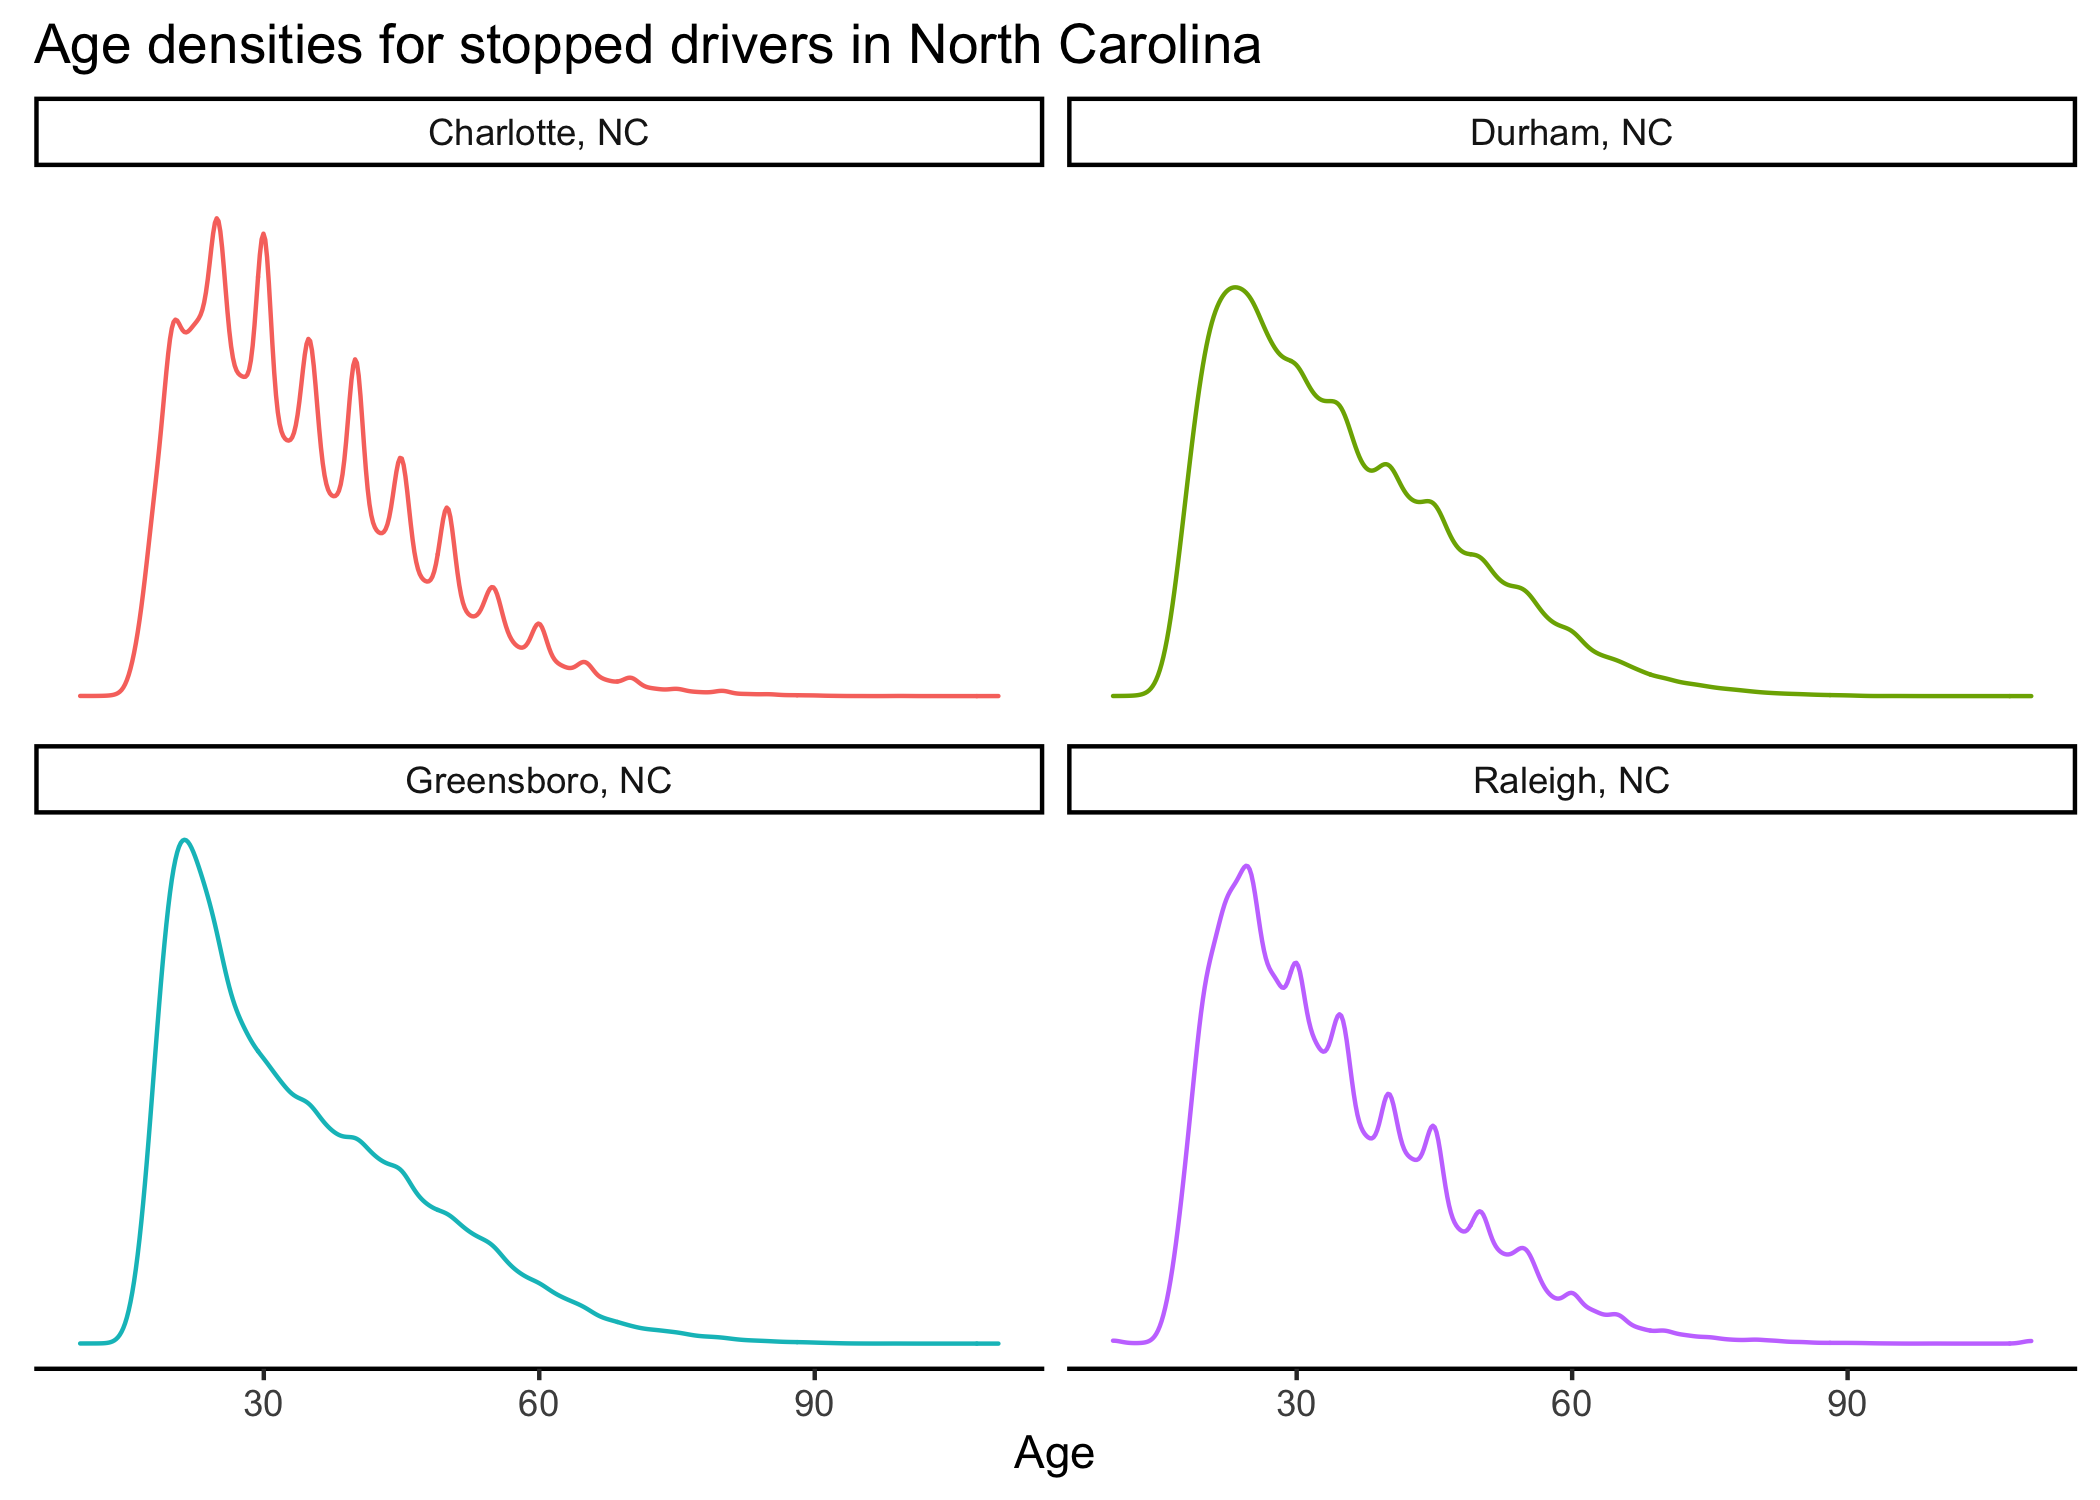
\includegraphics[scale=0.1]{fig/nc_age.png}
%	\end{center}
%	Evidently, North Carolina uses perception for age, too. 
%\end{frame}

\section{Visualizations}
\frame{\sectionpage}

\begin{frame}{SMR by race}
	\begin{center}
	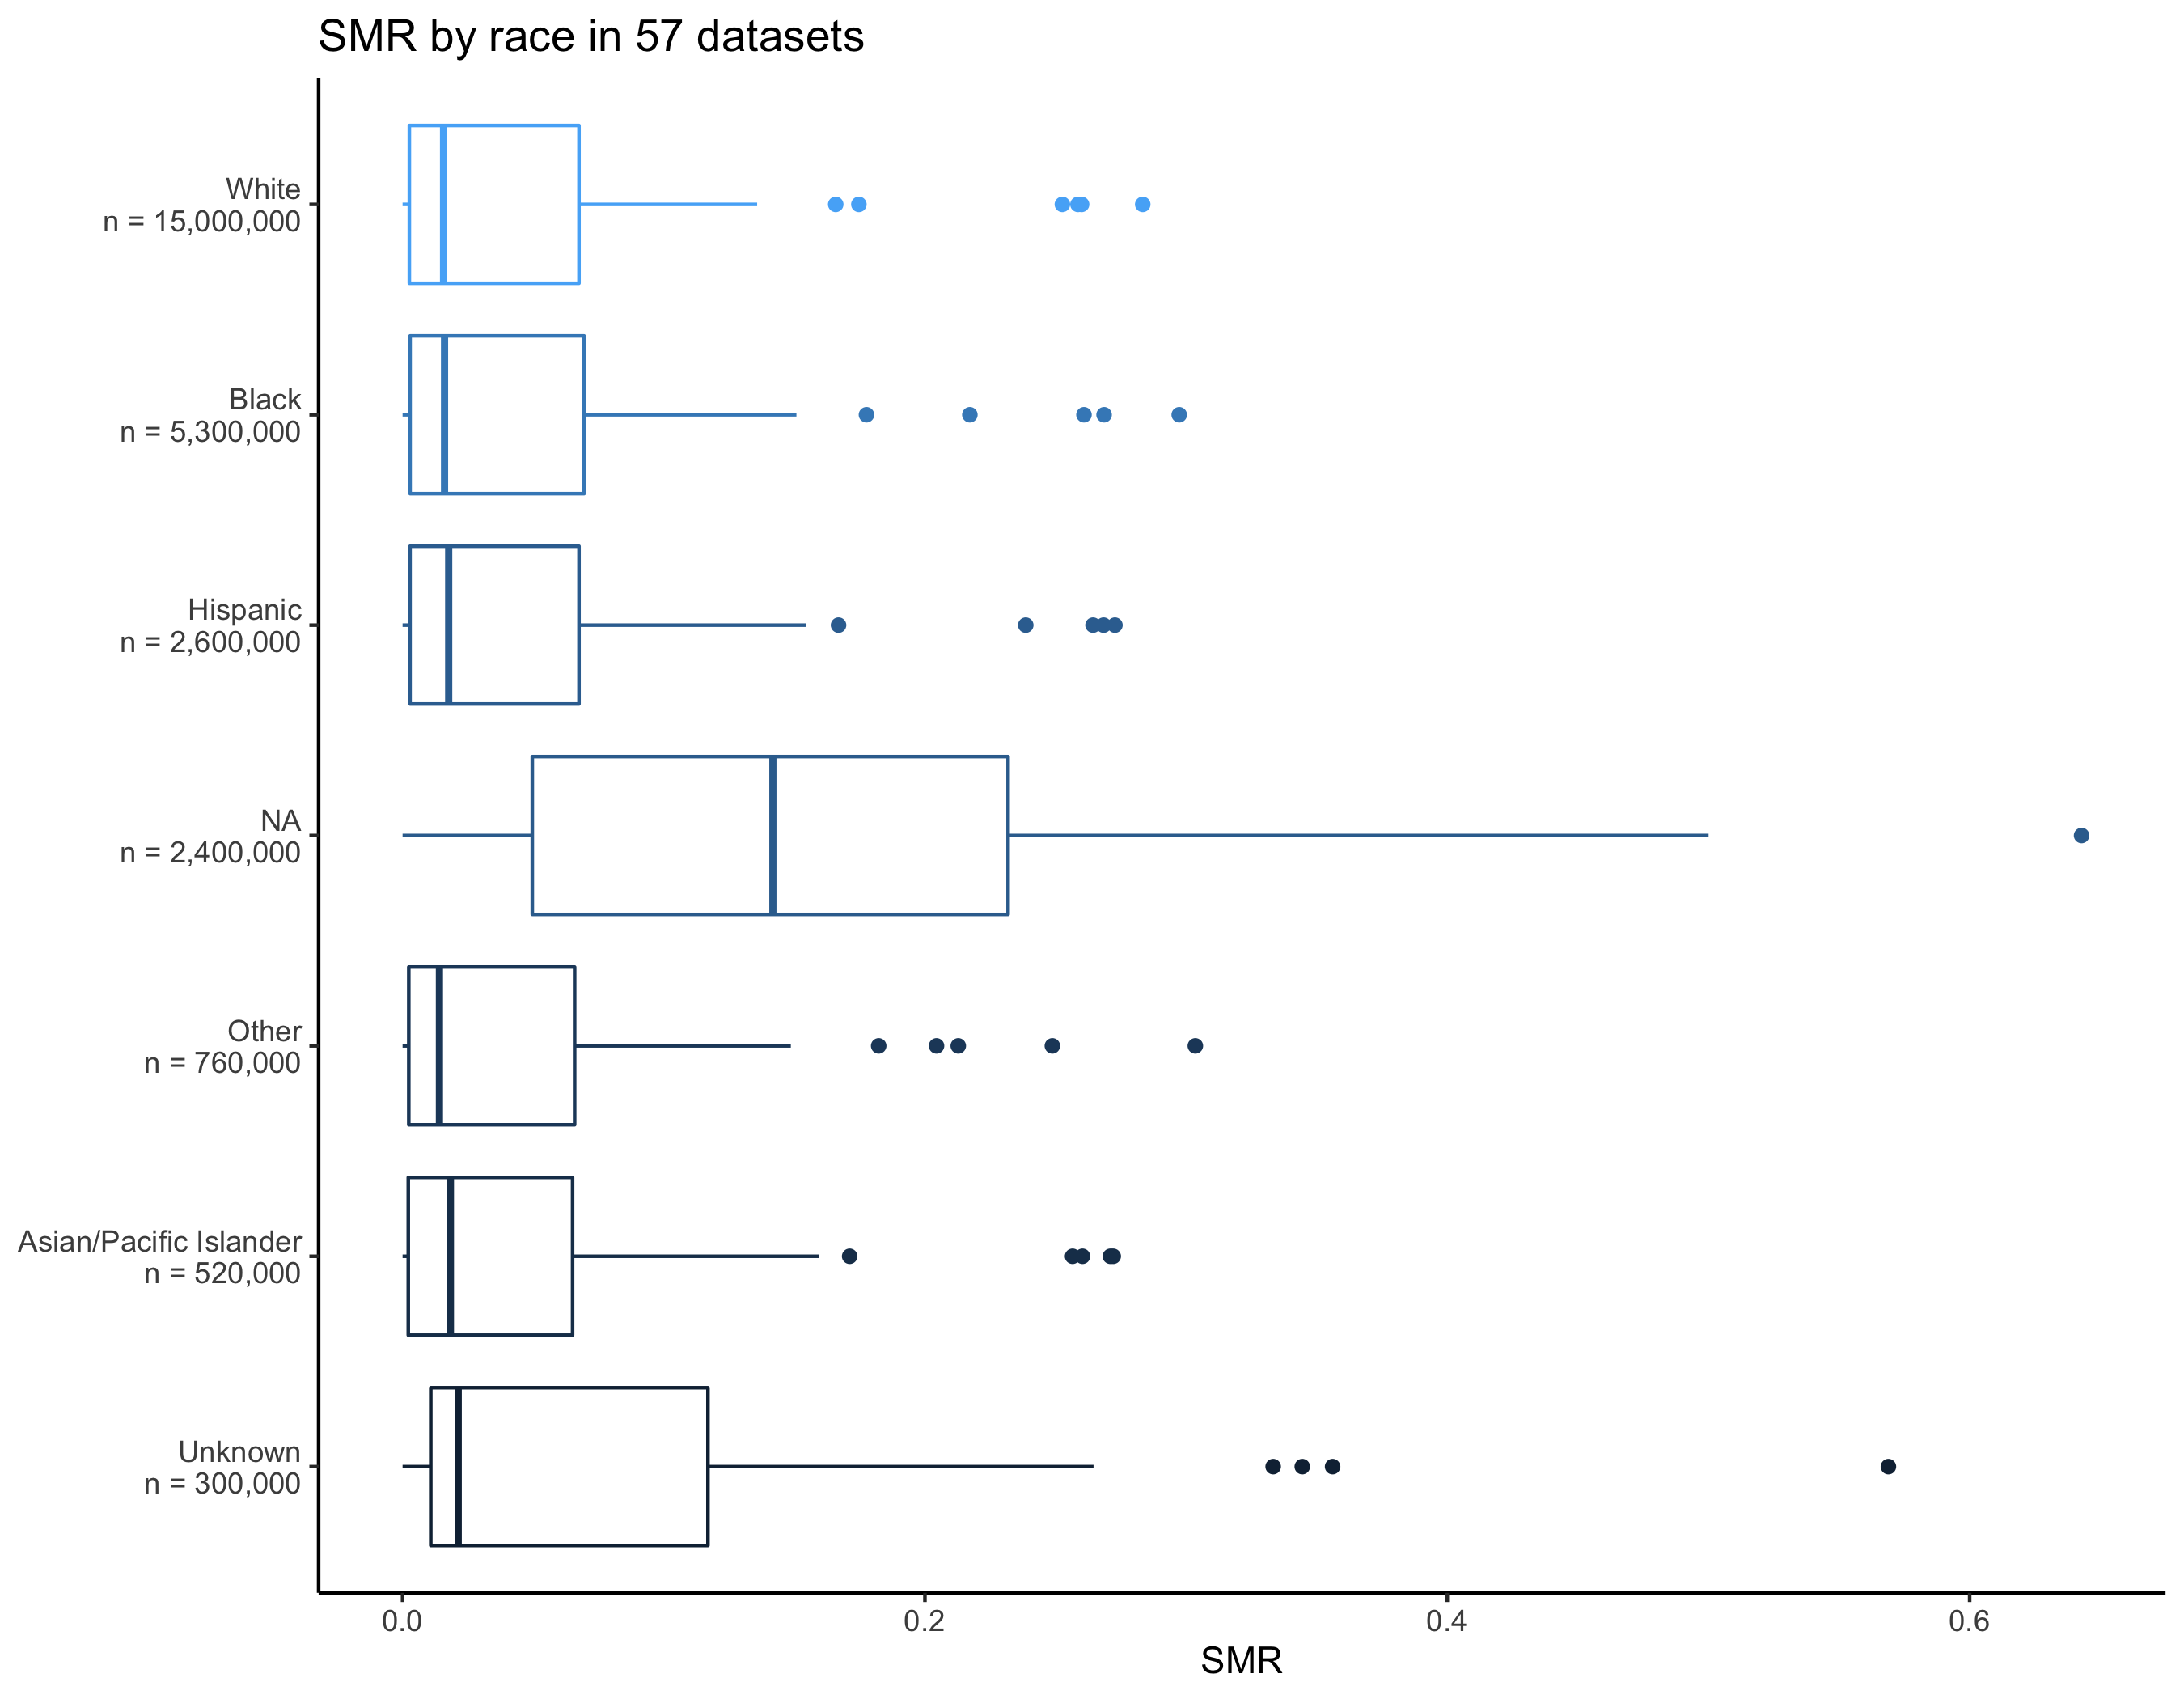
\includegraphics[scale=0.1]{fig/SMR_by_race.png}
	\end{center}
\end{frame}

\begin{frame}{SMR by race}
	\begin{center}
	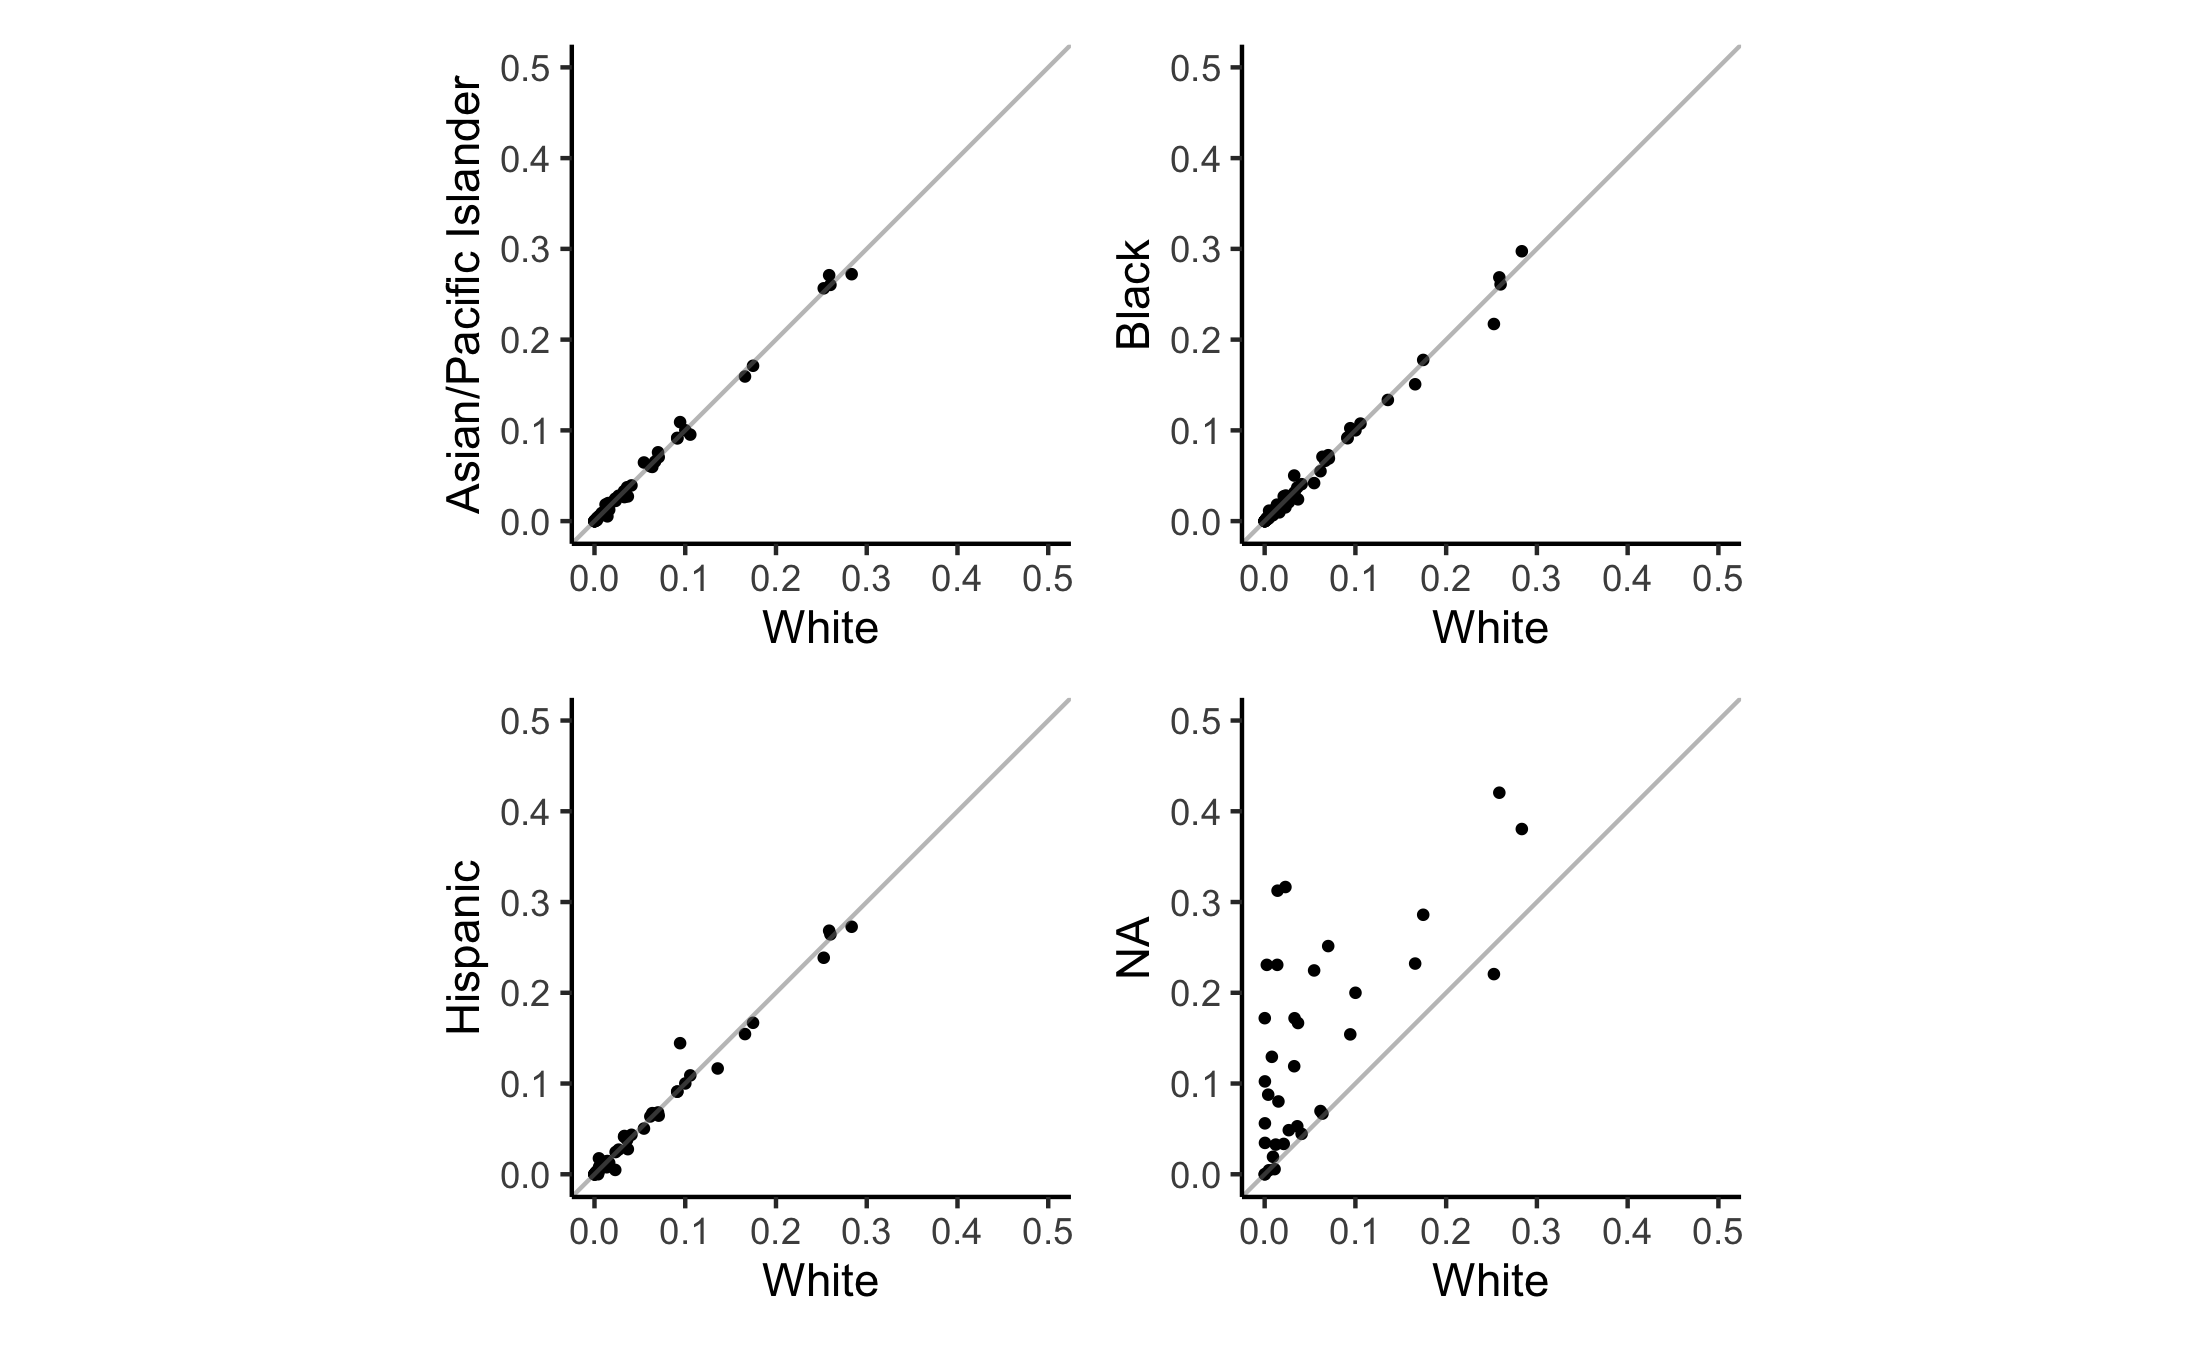
\includegraphics[scale=0.15]{fig/smr_race.png}
	\end{center}
\end{frame}

\begin{frame}{SMR by \texttt{date}}
	\begin{center}
	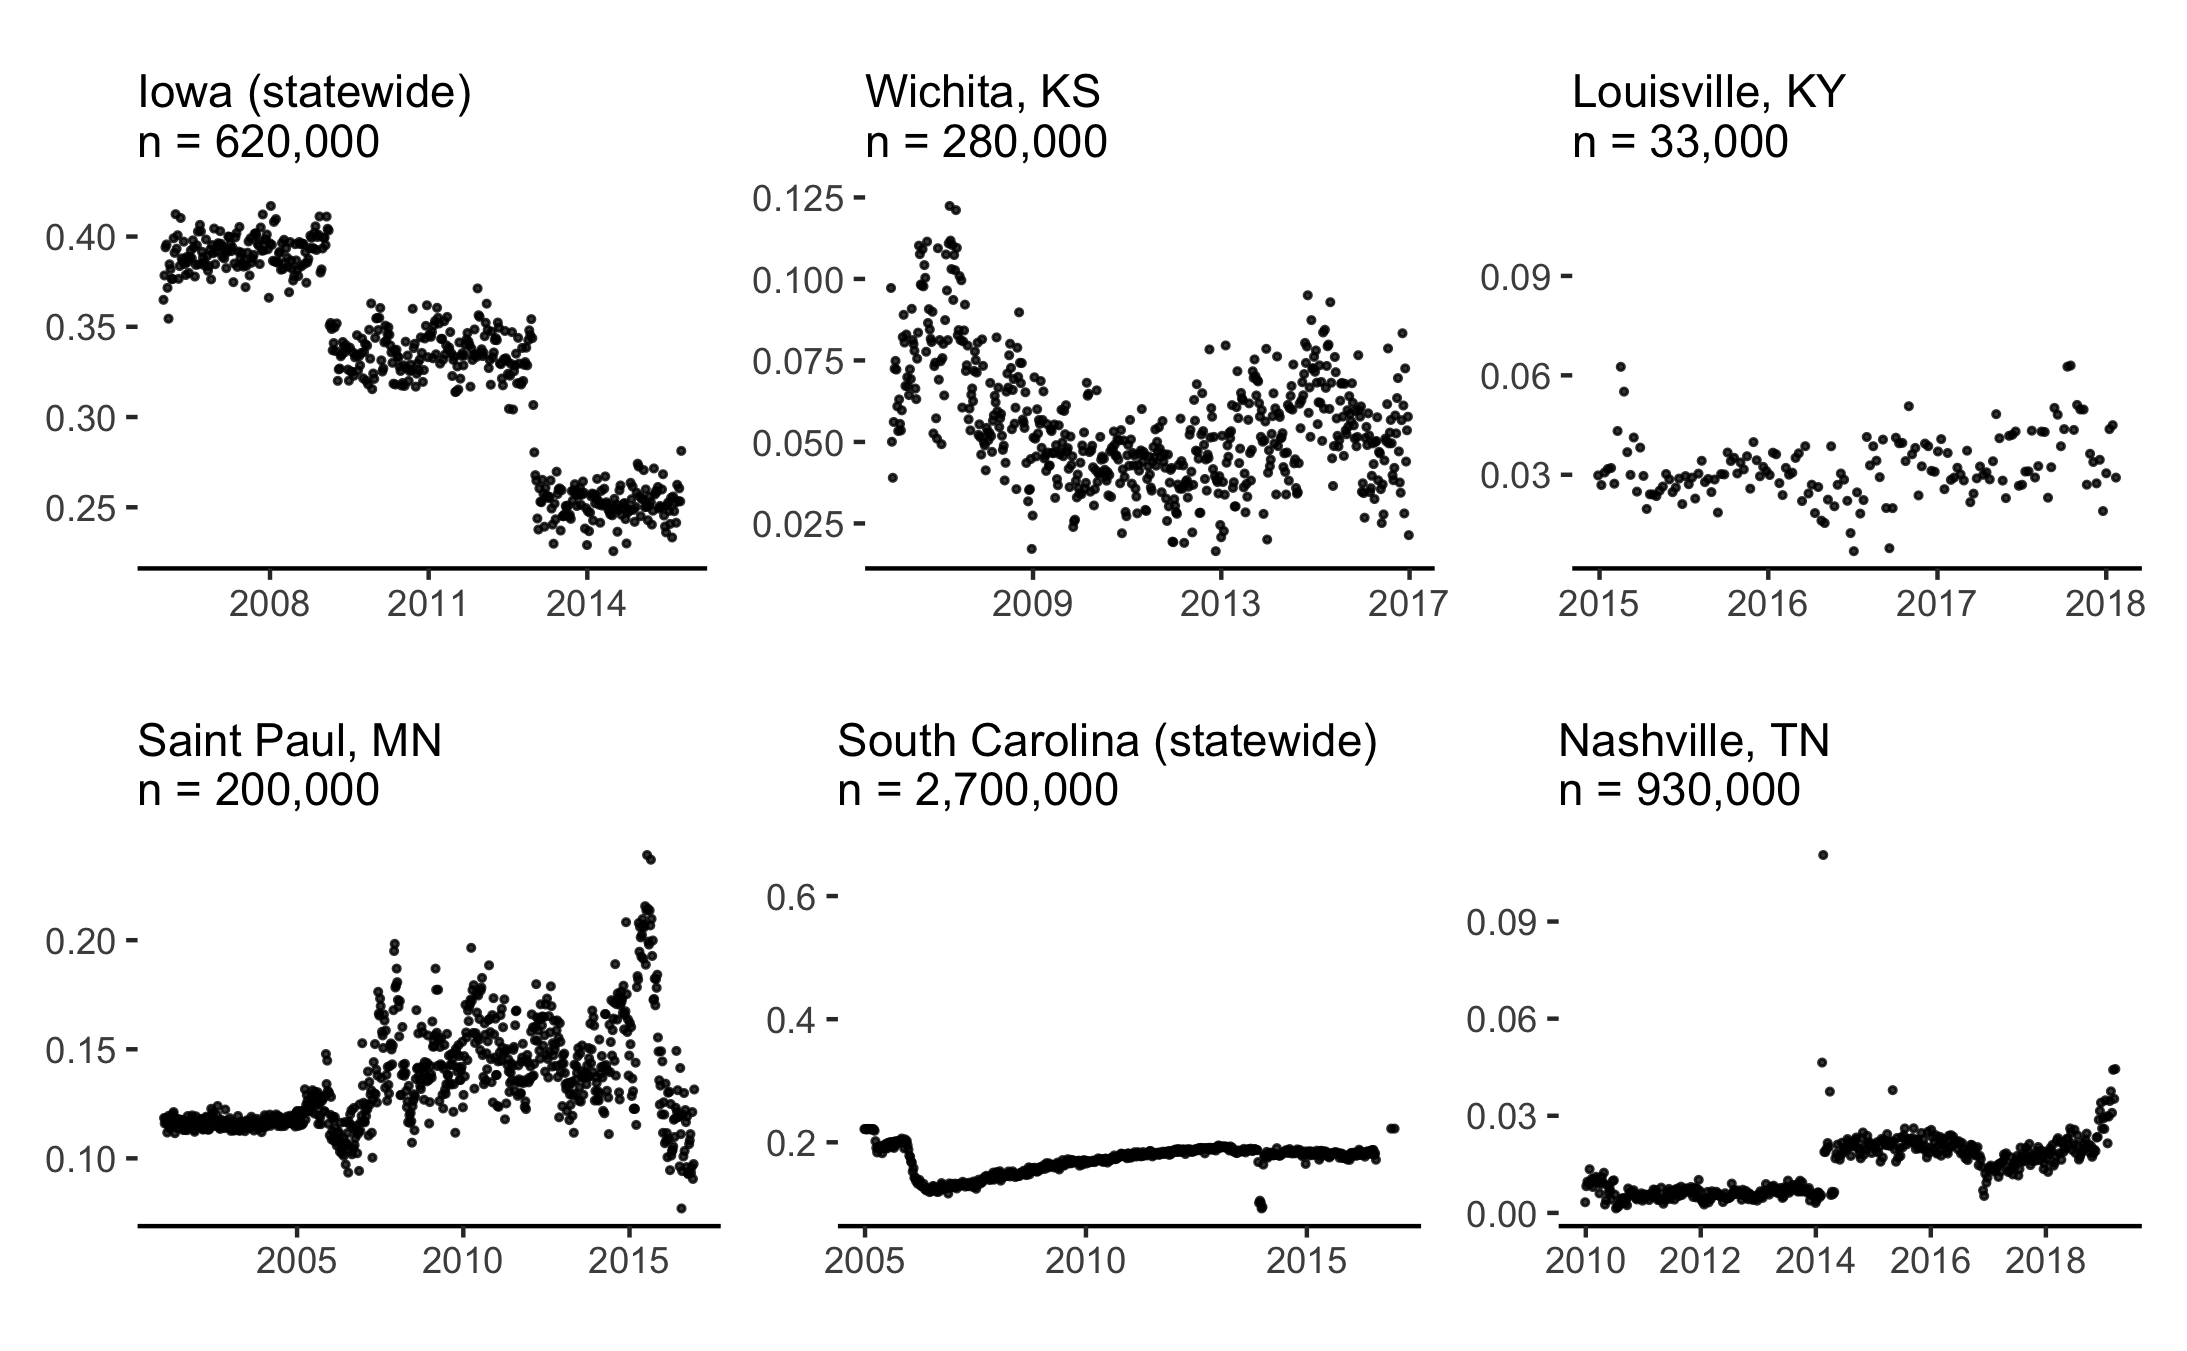
\includegraphics[scale=0.15]{fig/smr_temporal.png}
	\end{center}
\end{frame}

\begin{frame}{SMR by \texttt{time}}
	\begin{center}
	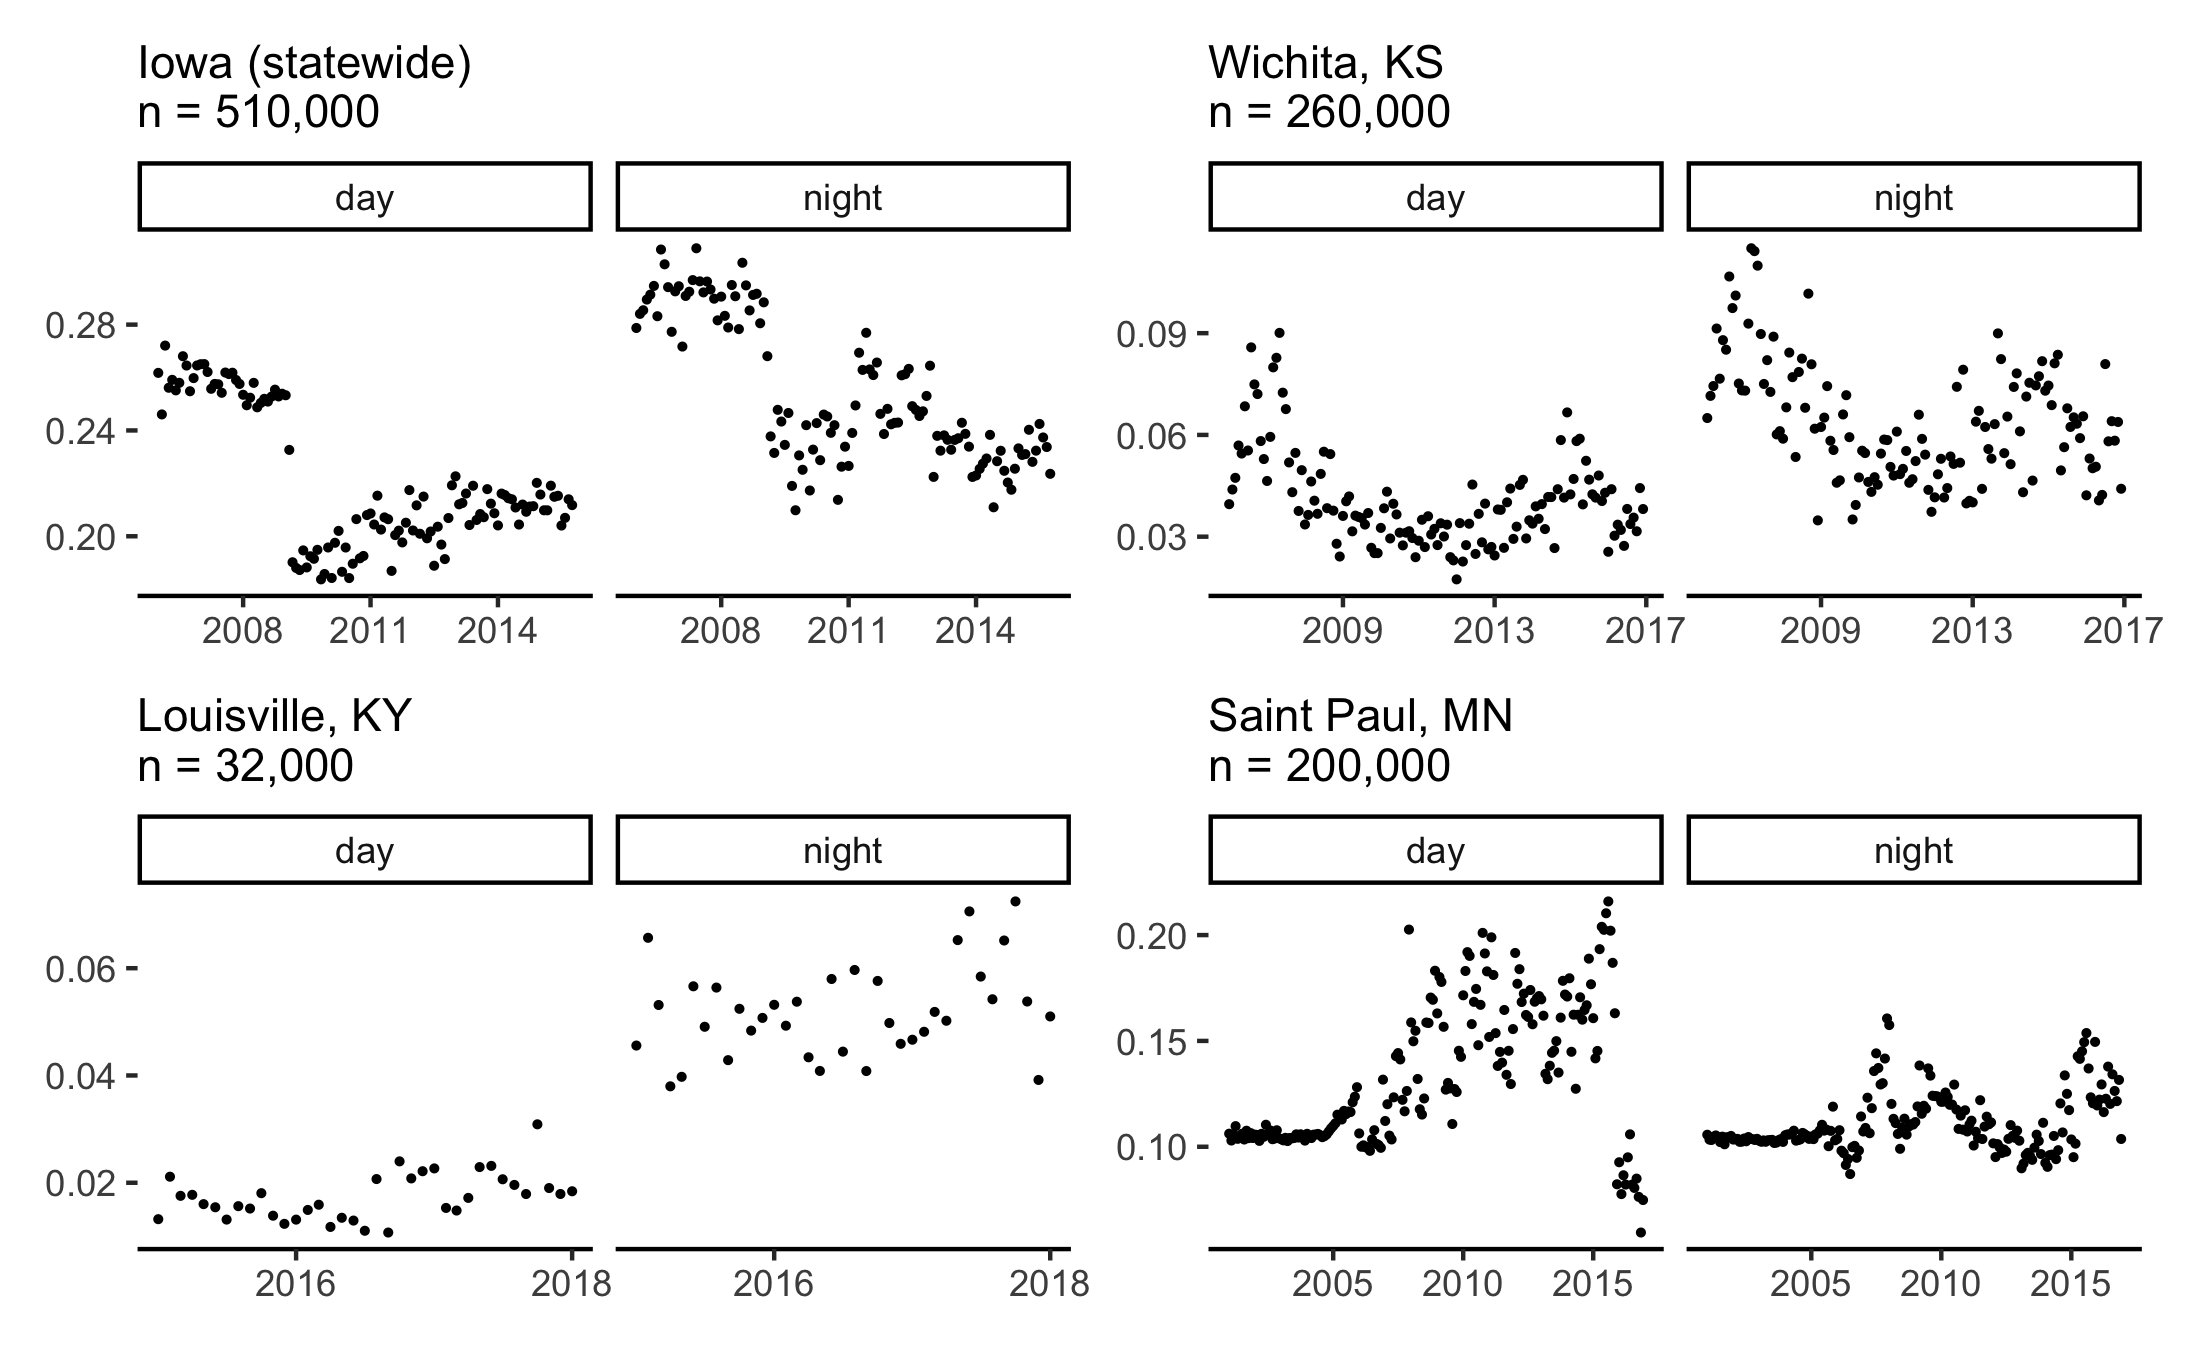
\includegraphics[scale=0.15]{fig/smr_daynnite.png}
	\end{center}
	% showing a few examples emblematic ...
	% artifically weighting traffic stops of a certain time period when excluding observations with missing values
\end{frame}

\begin{frame}{Discussion}
	\begin{itemize}
	\item Regarding \race, there isn't much evidence that Asian/Pacific Islander, Black, and Hispanic traffic stops are recorded differently than White traffic stops. 
	\item Traffic stops with missing \race \, have higher rates of missing values in other variables, too.
	\item Traffic stops are recorded differently based on the \texttt{date} and \texttt{time} of the traffic stop. Exactly \emph{how} the missingness is different depends on the dataset. 
	\item Future research could investigate the missingness mechanism (missing at random and missing not at random). 
	\end{itemize}
\end{frame}

\begin{frame}
	Thank you!
\end{frame}

\begin{frame}{Note: Data collection is a deeply human process.}
	In states like California and New York, officers use \emph{perception} to record driver race, gender, and age. 
	\begin{center}
	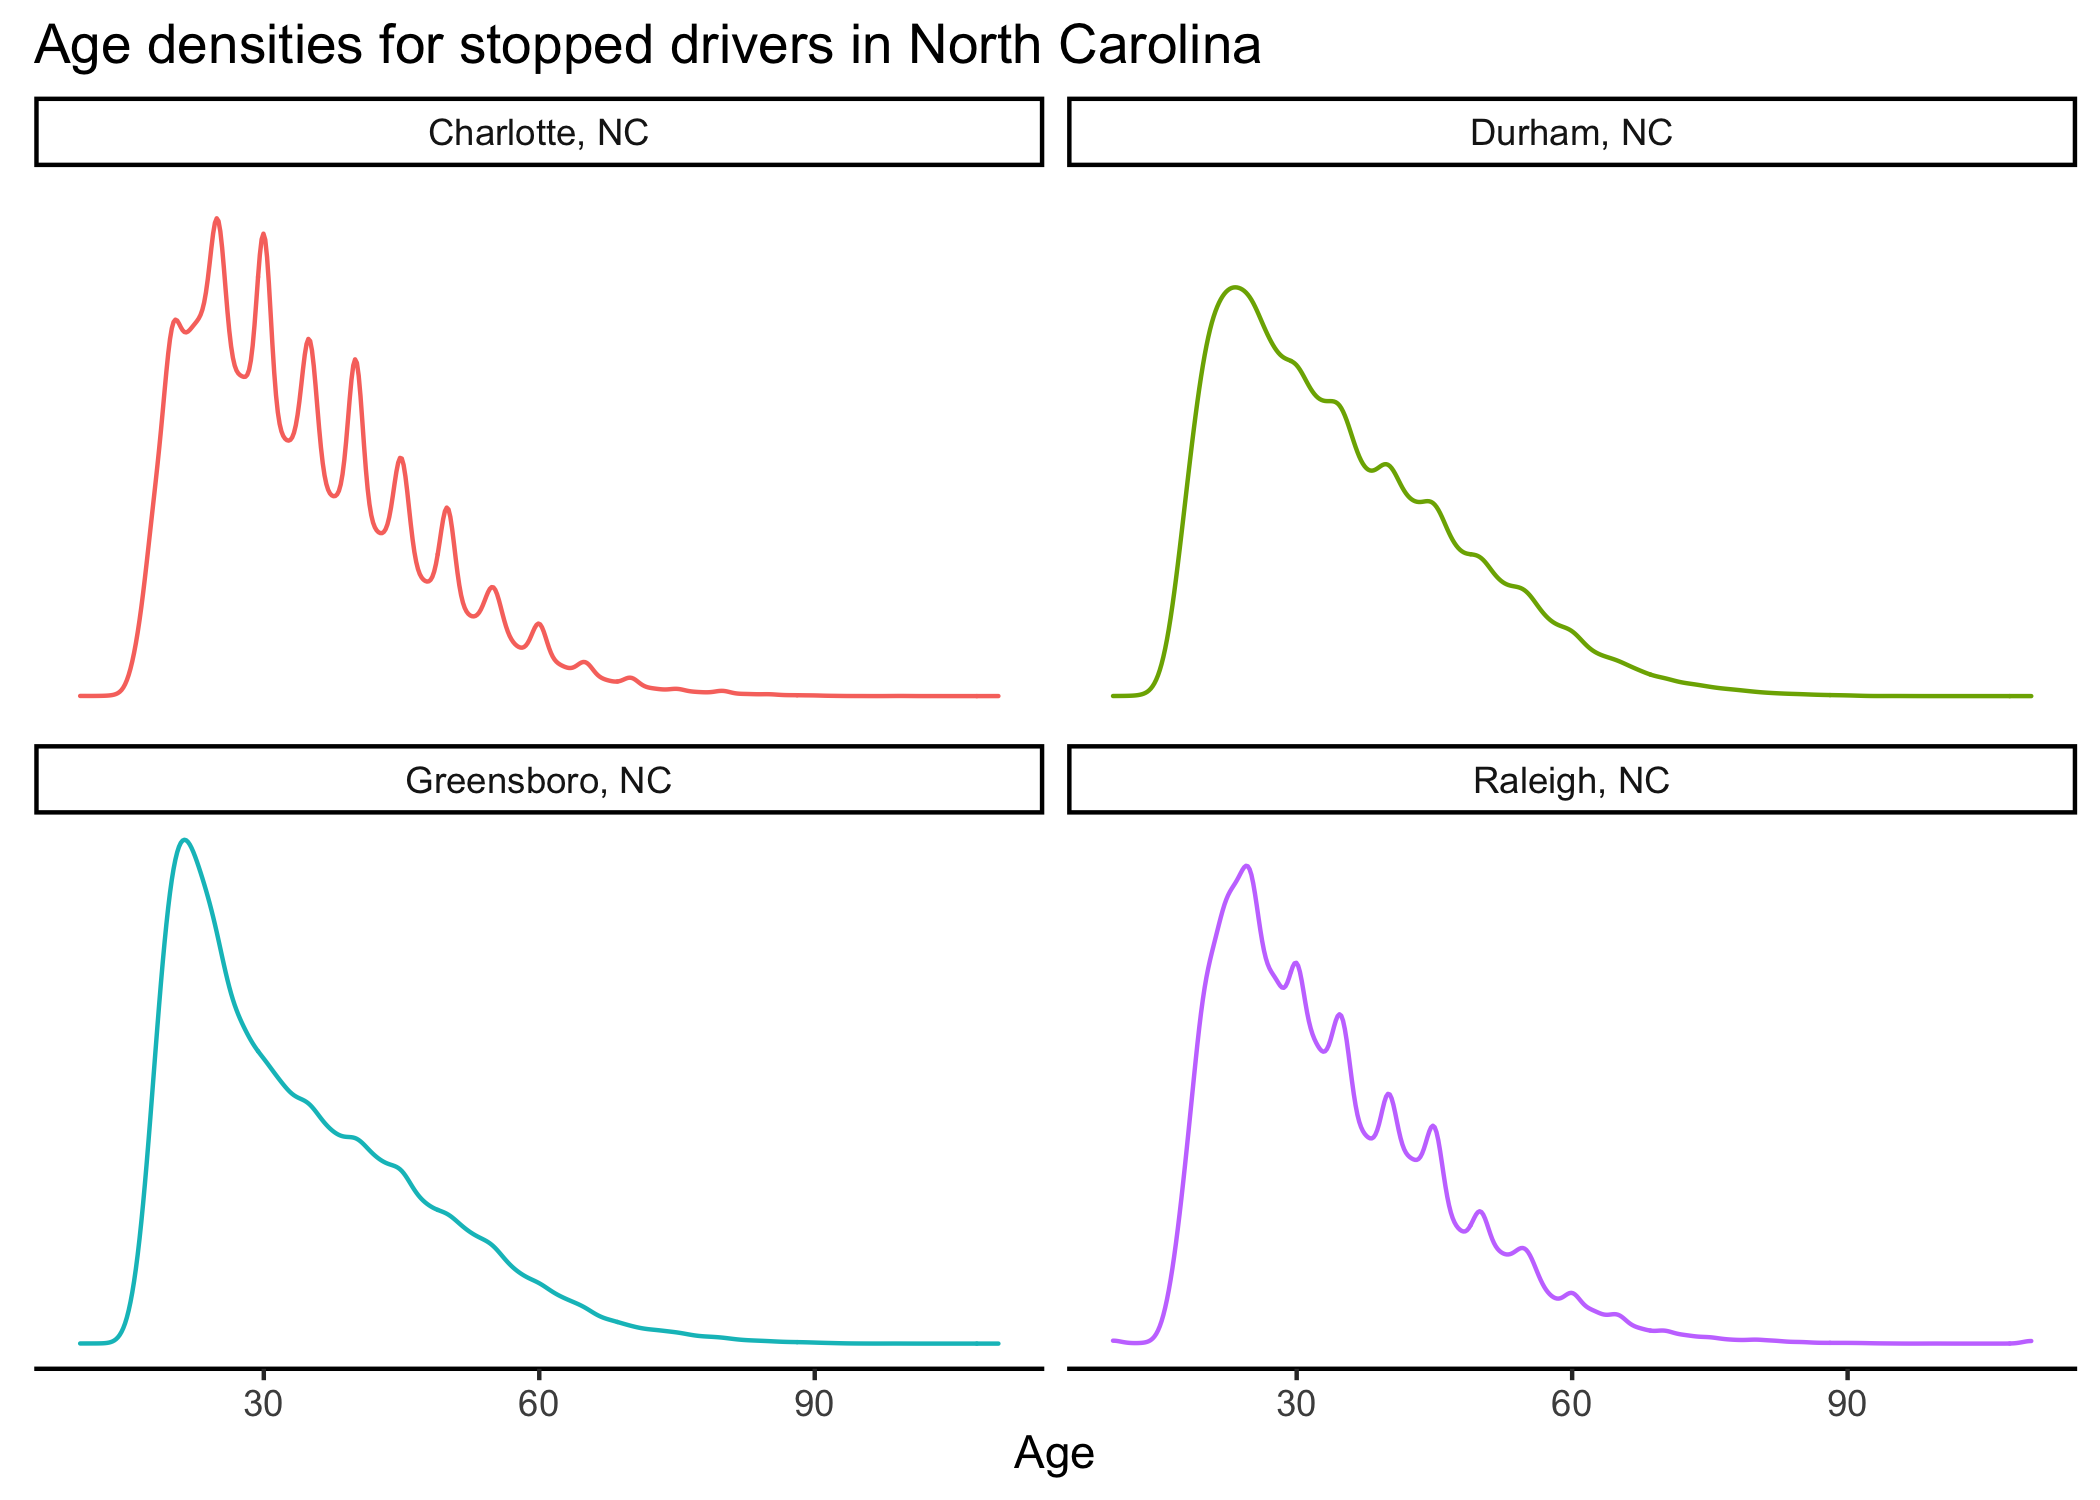
\includegraphics[scale=0.1]{fig/nc_age.png}
	\end{center}
	Evidently, North Carolina uses perception for age, too. 
\end{frame}


\iffalse

%===============================================================%
\section{First appendix section}
%===============================================================%

\begin{frame}{Appendix sample}

	Note that this slide doesn't count towards the total slides shown in the regular presentation

\end{frame}

\begin{frame}{hello}
    
\end{frame}
\fi
%===============================================================%
\end{document}
%===============================================================% 